\section{\change[\firstAuthorEdit]{SST Drivers of Heavy Rainfall Clustering}{Mechanisms associated with Heavy Rainfall Clustering}}
This section investigates the extent to which changes in the El Ni\~no-Southern Oscillation (ENSO) can explain changes in clustering\change{across timescales.}{, 
discuss whether top of the atmosphere radiative fluxes may positively feedback on the highly clustered states, 
and if a meridional clustering of heavy rainfall with warming is related to constraints on the tropical ascent area fraction.}

We use\add[\firstAuthorEdit]{
the Southern Oscillation Index \citep[SOI;][]{Ropelewski1987}} and the Oceanic Ni\~no Index \citep[ONI;][]{ONI_ref} 
to identify the state of the El Ni\~no-Southern Oscillation in interannual variability 
\add[\firstAuthorEdit]{and compare ascent area fraction, $A_a$, using the area where the 500 hPa vertical pressure velocity is negative. 
The SOI represents the standardized deseasonalized monthly anomalies of the surface pressure difference 
between Tahiti (17.6$^\circ{}$S, 149.6$^\circ{}$W) and Darwin (12.5$^\circ{}$S, 130.9$^\circ{}$E), 
calculated here as the three-month rolling average.} 
The ONI represents the three-month rolling average SST anomaly in the Ni\~no3.4 region (5$^\circ{}$S- 5$^\circ{}$N, 120$^\circ{}$-170$^\circ{}$W), 
calculated here relative to the full range of years used in the climatology.
\change[\firstAuthorEdit]{
ONI values greater than 0.5$^\circ{}$C represent El Ni\~no conditions and ONI values less than -0.5$^\circ{}$C represent La Ni\~na conditions. 
}{
SOI (ONI) values less (greater) than -7 (0.5) represent El Ni\~no conditions and SOI (ONI) values greater (less) than 7 (-0.5) represent La Ni\~na conditions.}
The climatological East-West Pacific SST gradient, defined as the time-mean difference between 
the SST in the western- (5$\degree$S - 5$\degree$N, 80$\degree$ - 150E) and eastern (5$\degree$S - 5$\degree$N, 180$\degree$ - 80$\degree$W) Pacific boxes, 
which we denote $T_z$, serves as an indicator for climatologically ``El Ni\~no-like'' conditions \citep{Watanabe2024}.

Observations show several indications that highly clustered states, corresponding to large values of the mean area of heavy precipitation features, $A_m$, 
are associated with El Ni\~no-like conditions \add[\firstAuthorEdit]{in interannual variability}. 
Firstly, \change[\firstAuthorEdit]{SST}{surface temperature} regressed onto $A_m$ \remove[\firstAuthorEdit]{for interannual variability}shows 
a pattern strongly reminiscent of an El Ni\~no SST signature \citep{Michael2002} (Figure \ref{mechanisms_obsMAP}). 
Secondly, during times of ONI exceeding 0.5$^\circ{}$C compared to all days, $A_m$ increases as heavy precipitation moves 
from the maritime continent towards the central Pacific (Figure S\change[\firstAuthorEdit]{7b}{6} in supporting information).
Finally, \add[\firstAuthorEdit]{in absolute value} and independent of changes in \change[\firstAuthorEdit]{$A_f$}{$C$}, \add[\firstAuthorEdit]{SOI} and ONI show\remove[\firstAuthorEdit]{s} 
a \change[\firstAuthorEdit]{positive}{negative (positive)} correlation with $A_m$ (Figure \ref{mechanisms_obsSCATTER}a \add[\firstAuthorEdit]{and Figure S1 in supporting information}).
\add[\firstAuthorEdit]{From qualitatively analysing snapshots of observed precipitation features from the climatology of individual months during El Ni\~no and La Ni\~na conditions (interannual variability), 
a greater mean area of heavy rainfall is favoured during El Ni\~no conditions due to a greater total area coverage of heavy precipitation locally growing precipitation features 
in combination with more frequently forming large connected components (precipitation features) in the central Pacific (ex: Figure 1c).
}From these results, we may argue ENSO as a driver for interannual variability in clustering, however, it is possible that radiative effects 
associated with clustering may feedback on its development and maintenance. Initial investigation suggest such radiative feedbacks are present 
and may contribute to amplifying the existing pattern of the frequency of occurence of heavy precipitation associated with the highly clustered states 
(Figure S7 in supporting information).

Most CMIP models capture the observed connection between \change[\firstAuthorEdit]{ONI}{SOI} and $A_m$ (Figure S1 in the supporting information) and
the independent contribution of \change[\firstAuthorEdit]{ONI}{SOI} on $A_m$ outside the influence of \change[\firstAuthorEdit]{$A_f$}{$C$}, as does the high-resolution GCM 
(\remove[\firstAuthorEdit]{Figure S3 in the supporting information and}Figure \ref{mechanisms_obsSCATTER}b). 
Thus both models and observations show that large-scale clustering of precipitation is \change[\firstAuthorEdit]{stronger}{greater} 
during El Ni\~no than La Ni\~na \add[\firstAuthorEdit]{in interannual variability}. This is despite the fact that El Ni\~no represents a weakening of the Walker circulation 
and a weakening of tropical SST gradients, both of which are generally thought to facilitate the organization of convection on large scales.

\add[\firstAuthorEdit]{
The interpretation as to whether large-scale clustering is favoured during El Ni\~no events will be sensitive to whether clustering is interpreted as 
increasing or decreasing with total area coverage of heavy precipitation, $C$, for example when using $N$ instead of $A_m$, 
and may be sensitive to the temporal and spatial resolution of the precipitation dataset as well as the clustering metric used.
Notably, from idealized SST perturbed GCM experiments Quan et al. in 2025 find "La Ni\~na" like conditions favour highly clustered states on the large scale, but 
target increases in "uneveness", or precipitation gradients, as large-scale clustering (GINI index).
Still, in observed and modelled interannual variability in the present study the GINI index is somewhat negatively correlated with SOI (r$\sim$-0.15- -0.4),
indicating more El Ni\~no like conditions favour highly clustered states (Figure S1 in supporting information).
We suspect the diverging results is due to how the ENSO related SST pattern manifest naturally compared to when experimentally imposed, for example including a 
"horseshoe" shaped relative cooling in the Pacific in natural variability during El Ni\~no events. However, this interpretation is tentative and requires further investigation.
}

\clearpage
\begin{figure}
    \centering
    \includegraphics{sections/result_2/figures/linear_regression_map_tas.pdf}
    \caption{NOAA-GlobalTemp surface temperature \add[\firstAuthorEdit]{(land and ocean)}, $T_s$, 
    regressed onto $A_m$ for interannual variability. 
    The contour shows the climatological 90th percentile of $T_s$, 
    and crosses indicate whether correlations are statistically significant.}
\label{mechanisms_obsMAP}
\end{figure}

\begin{figure}
    \centering
    \includegraphics{sections/result_2/figures/scatter_and_box_soi.pdf}
    \caption{Same as Figure 3, 
    but with the \change[\firstAuthorEdit]{Oceanic Ni\~no Index (ONI)}{Southern Oscillantion Index (SOI)} in scatter colors 
    and as explanatory variable in boxplot.}
\label{mechanisms_obsSCATTER}
\end{figure}
\clearpage

The strong connection between El Ni\~no conditions and \change[\firstAuthorEdit]{$A_m$}{clustering} in interannual variability 
motivates the investigation of changes in the climatological Pacific SST gradient to a more El Ni\~no-like state as a mechanism 
for explaining model-spread in projected changes in clustering. Consistent with expectations, the magnitude of the weakening of the East-West Pacific SST gradient 
explains a similar amount of variance in projected changes in clustering as the zonal shift in heavy precipitation (Figure \ref{mechanisms_warmingSCATTER}). 
Models that have more El Ni\~no-like warming patterns tend to exhibit larger increases in large-scale clustering of precipitation. 
Regressing the SST changes against projected changes in the mean area of precipitation features, $A_m$, also shows an El-Ni\~no-like pattern, 
with a relative warming in the east and relative cooling in the west (Figure \ref{mechanisms_warmingMAP}). 
In addition, the regression pattern has a noticeable north-south gradient, 
consistent with the positive regression coefficients for heavy precipitation frequency north of the equator in 
Figure \ref{spatial_preference_warmingMAP}. 

\clearpage
\begin{figure}
    \centering
    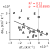
\includegraphics{sections/result_2/figures/clim_change_scatter_Tz.pdf}
    \caption{Same as Figure 4a, 
    but with the change in the climatological Pacific SST gradient, $T_z$, per Kelvin tropical warming from the historical to the SSP585 scenario simulation period across the CMIP6 ensemble as explanatory variable. 
    Models are as given in the legend in Figure 4.}
\label{mechanisms_warmingSCATTER}
\end{figure}

\begin{figure}
    \centering
    \includegraphics{sections/result_2/figures/linear_regression_change_tas.pdf}
    \caption{Change in surface temperature, $T_s$, 
    regressed onto change in mean area of heavy precipitation features, $A_m$, per Kelvin tropical warming from the historical to the SSP585 scenario simulation period across the CMIP6 ensemble. 
    Contour shows ensemble-mean 90th percentile climatological $T_s$ and crosses indicate if correlations are statistically significant.}
\label{mechanisms_warmingMAP}
\end{figure}
\clearpage

\add[\firstAuthorEdit]{
Note, while changes to the Pacific SST gradient may be climatologically argued as a driver for changes in clustering with warming 
there are changes in the zonal SST gradient, $T_z$, and the mean distance of heavy precipitation to the central Pacific 
of both signs across the 27 CMIP6 models we analyse, suggesting that zonal shifts in convection are not the primary reason 
for the ensemble-mean increase in large-scale clustering with warming that we document. We hypothesize that the ensemble-mean increase in $A_m$ 
is instead associated with a meridional shift in convection. All but one model increase proximity of heavy precipitation 
to the geographic and hydrological equator with warming, and this is associated with an increase in the large-scale clustering of precipitation in natural variability.
The increased proximity of heavy precipitation to the hydrological equator with warming can be interpreted as a meridional clustering of convection to the centre of the ITCZ, or a ``narrowing'' of the ITCZ. 
Mechanistically, changes to the ``width'' or area of the ITCZ characterized by changes in the tropical ascent area fraction relative to descent area fraction
is theorized to be controlled by convective limitations on the efficiency of moisture and heat export from the ITCZ to its surroundings (the Gross Moist Stability) \citep{Byrne2016}. 
From this framework, the forced response to global warming modulate the ``width'' (or area) of the ITCZ to maintain the energy balance between regions of 
ascent and descent. While the narrowing tendency is a combination of ascent area reduction and descent area expansion, 
a reasonably strong relationship between ascent area fraction, $A_a$, and proximity of heavy rainfall to the hydrological equator, $P_{heq}$, 
(Figure \ref{mechanisms_warmingSCATTER2}) support the notion of a mechanistic connection to aspects of large-scale clustering of heavy precipitation.
}

\clearpage
\begin{figure}
    \centering
    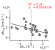
\includegraphics{sections/result_2/figures/clim_change_scatter_cheq_Aa}
    \caption{Same as Figure 4a, 
    but with the change in climatological area of ascent, $A_a$, per Kelvin tropical warming from the historical to the SSP585 scenario simulation period across the CMIP6 ensemble as explanatory variable. 
    Here, the climatological area of ascent is calculated as the climatological time-mean of the fraction of the tropical domain where the monthly-mean 500hpa vertical pressure velocity in negative.
    Models are as given in the legend in Figure 4.}
\label{mechanisms_warmingSCATTER2}
\end{figure}

\add[\firstAuthorEdit]{In this section} we have shown that El Ni\~no-like states tend to result in a higher degree of clustering 
in both interannual variability and across the CMIP6 ensemble under climate change, 
\remove[\firstAuthorEdit]{
Note, however, that there are changes in the zonal SST gradient, $T_z$, 
and the mean distance of heavy precipitation to the central Pacific of both signs across the 27 CMIP6 models we analyse, 
suggesting that zonal shifts in convection are not the primary reason for the ensemble-mean increase in large-scale clustering with warming that we document. 
All but one model exhibit negative changes in $C_m$ with warming, 
and this is associated with an increase in the large-scale clustering of precipitation in natural variability.
}
but highlight cloud-radiative feedbacks and energetic constraints on the large-scale circulation of moisture and heat \citep{Byrne2016} may influence the manifestation of clustering 
in interannual variability and for climatological changes with warming, respectively. In the next section, 
we explore the tropical humidity and cloud distributions associated with clustered states and how it relates to climate sensitivity.


% As highlighted in the previous section, 
% in a climatological comparison of the spatial preference across models (Figure S5), while not directly related to a climatologically greater Pacific SST gradient, 
% heavy precipitation occur more frequently over the maritime continent and SPCZ region in models with climatologically larger clustering.

% Quan et al. quantify clustering based on a relative dispersion measure, or "uneveness", of the precipitation distribution (GINI index) 
% and find relatively heating the top 30 percent warmest regions (greater east-west Pacific SST gradient) increase the clustering metric and reduce the area of ascent.

